\section{Desarrollo del núcleo formal: condiciones iniciales, geometría y refinamiento}
\label{sec:extension}

El soporte de ochenta y una posiciones no coincide con el dominio de condiciones iniciales de la dinámica. Una condición inicial debe indicar además una orientación; y las hojas aditiva y multiplicativa disponen de cursores independientes. Esta distinción permite reconstruir exhaustivamente la emisión sin seleccionar de antemano una región numérica.

\subsection{Los estados iniciales y la recurrencia de emisión}

Para la enumeración utilizamos índices \(I_9=\{0,\ldots,8\}\), relacionados con las etiquetas positivas por \(i\mapsto i+1\). Sea
\[
 \mathcal S=I_9^2\times\{N,E,S,O\},\qquad
 \Omega_{\rm seed}=\mathcal S_+\times\mathcal S_\times.
\]
Cada condición inicial \(\omega=(s_+,s_\times)\) determina dos posiciones y dos direcciones. El dominio comprende todas las parejas ordenadas, por lo que
\begin{equation}
 |\mathcal S|=324,\qquad |\Omega_{\rm seed}|=324^2=104\,976.
 \label{eq:semillas}
\end{equation}
La parametrización anterior ya es una enumeración interna: cada uno de los
\(81\) pares de posiciones aparece con las cuatro direcciones, y el producto
cartesiano conserva las \(324^2\) combinaciones de los dos cursores. Las filas
de una tabla de emisiones son fibras de este dominio de condiciones iniciales;
no se añade un catálogo exterior para definirlas.

La realización finita utiliza seis ventanas de nueve transiciones. En cada instante \(t\), la firma de fase es \(M_{\rm ph}(1+((t-1)\bmod9))\). Si vale \(+1\), se lee el residuo positivo \(\Sigma(i+1,j+1)=\rho_9(i+j+2)\) del primer cursor y después se desplaza ese cursor; si vale \(-1\), se lee el residuo positivo \(\Pi(i+1,j+1)=\rho_9((i+1)(j+1))\) del segundo cursor y después se desplaza el segundo. El valor cero incrementa el contador neutral. Al finalizar las transiciones veintisiete y cincuenta y cuatro, se invierten las orientaciones cardinales. Las evaluaciones enteras y sus cocientes se conservan en el registro, pero el emisor utiliza las lecturas residuales aquí especificadas.

En el sector de unidades, el lector multiplicativo utiliza el logaritmo discreto de base dos en \((\ZZ/9\ZZ)^\times\):
\[
 \ell_9(1)=0,\quad\ell_9(2)=1,\quad\ell_9(4)=2,\quad
 \ell_9(8)=3,\quad\ell_9(7)=4,\quad\ell_9(5)=5.
\]
Para la emisión finita se extiende con valor cero al sector no unitario. Esta extensión es un observable y no una identificación de los elementos \(3,6,9\) con la unidad multiplicativa. La hoja y su pertenencia al sector radical permanecen en el registro de trayectoria.

Sean \(S_m\) la suma de los tres residuos positivos aditivos \(\Sigma\) de la ventana \(m\), \(E_m\) la suma de los tres exponentes discretos de los residuos multiplicativos \(\Pi\) y \(Z_m=3\) el número de eventos neutrales. Así, \(S_m\) no suma las evaluaciones enteras \(S=i+j\), cuyos cocientes permanecen en el registro. Con \([a]_{10}\in\{0,\ldots,9\}\), la regla de emisión decimal es
\begin{align}
 d_{m,1}&=[S_m]_{10},\notag\\
 d_{m,2}&=[S_m+E_m]_{10},\notag\\
 d_{m,3}&=[3S_m+5E_m+7Z_m]_{10},\notag\\
 U_m&=100d_{m,1}+10d_{m,2}+d_{m,3}.
 \label{eq:emisor-seis}
\end{align}
Los coeficientes enteros y el calendario de esta recurrencia son parte explícita de la ley emisora declarada. No se reciben valores de \(\pi,\varphi,e\) ni de \(\alpha\). La distinción entre una regla de emisión y una constante reconocida a partir de su salida evita que la genealogía quede escondida en una tabla de decimales.

Si \(s_m=[S_m]_{10}\) y \(e_m=[E_m]_{10}\), la misma regla se escribe
\begin{equation}
 U_m=100s_m+10[s_m+e_m]_{10}+[3s_m+5e_m+1]_{10}.
 \label{eq:acoplamiento}
\end{equation}
El uno final es el residuo de \(7Z_m=21\) módulo diez. La reducción ternaria orientada del catálogo adopta la convención
\begin{equation}
 \Psi(U_1,\ldots,U_6)=([-U_1]_3,\ldots,[-U_6]_3).
 \label{eq:psi-catalogo}
\end{equation}
El signo de esta coordenatización es explícito: cambiarlo modifica las palabras y exige transportar las orientaciones posteriores. La identificación balanceada de cada componente de \(\FF_3\) con el TRIT se realiza después de \eqref{eq:psi-catalogo}.

\begin{lemma}[Censo completo de las firmas de cursor]
\label{lem:censo-interno-firmas}
Las \(324\) condiciones iniciales de cada cursor se distribuyen en dieciocho
firmas aditivas de cardinal \(18\) y veintiséis firmas multiplicativas: una
de cardinal \(108\), una de cardinal \(24\) y veinticuatro de cardinal \(8\).
Estos cardinales y las firmas se obtienen de las reglas del emisor, sin
consultar valores reales ni tablas de constantes.
\end{lemma}
\begin{proof}
Identifiquemos las direcciones con
\[
 v_N=(-1,0),\quad v_E=(0,1),\quad
 v_S=(1,0),\quad v_O=(0,-1)
 \qquad\text{en }(\ZZ/9\ZZ)^2.
\]
En la hoja aditiva, la firma sólo depende de
\(c=i+j\pmod9\) y del sentido
\(\epsilon(d)=+\) para \(d\in\{E,S\}\),
\(\epsilon(d)=-\) para \(d\in\{N,O\}\). Para cada par
\((c,\epsilon)\) hay nueve elecciones de \(i\), que fijan \(j=c-i\), y
dos direcciones del sentido indicado. Por tanto, cada fibra contiene
\(9\cdot2=18\) semillas. La sustitución en las seis ventanas da la tabla
completa
\[
\begin{array}{c|cc}
c&\epsilon=-&\epsilon=+\\ \hline
0&212988&988212\\
1&645212&212645\\
2&988546&546988\\
3&221889&889221\\
4&564122&122564\\
5&898465&465898\\
6&122898&898122\\
7&456221&221456\\
8&889654&654889
\end{array}
\tag{A}
\label{eq:tabla-firmas-aditivas}
\]
y sus fibras son, explícitamente,
\[
 \mathcal P_{c,+}=\{(i,c-i,d):i\in\ZZ/9\ZZ,\ d\in\{E,S\}\},
 \quad
 \mathcal P_{c,-}=\{(i,c-i,d):i\in\ZZ/9\ZZ,\ d\in\{N,O\}\}.
\]

Para la hoja multiplicativa, escribamos
\(M(a,b)=\rho_9((a+1)(b+1))\) y, para \(m=0,\ldots,5\), \(r=0,1,2\),
\[
 a_{m,r}=\begin{cases}
 3m+r,&0\le m\le2,\\
 -(3(m-3)+r),&3\le m\le5.
 \end{cases}
\]
La firma de \(T=(i,j,d)\) queda determinada, componente a componente, por
\begin{equation}
 e_m(T)=\left[\sum_{r=0}^{2}
 \ell_9\!\left(M\bigl((i,j)+a_{m,r}v_d\bigr)\right)\right]_{10}.
 \label{eq:generador-firmas-multiplicativas}
\end{equation}
Esta expresión contiene las \(81\cdot4=324\) sustituciones posibles. La
clasificación exhaustiva de sus valores es
\[
\begin{array}{c|c|c}
\text{firmas}&\text{número de firmas}&\text{cardinal de cada fibra}\\ \hline
000000&1&108\\
555555&1&24\\
\begin{gathered}
177393,177555,177771,339555,339771,339933,\\
393177,393393,393555,555177,555339,555393,\\
555717,555771,555933,717555,717717,717933,\\
771177,771339,771555,933339,933555,933717
\end{gathered}&24&8
\end{array}
\tag{B}
\label{eq:tabla-firmas-multiplicativas}
\]
Cada entrada de (B) se verifica sustituyendo \(i,j\in\{0,\ldots,8\}\) y
las cuatro direcciones en \eqref{eq:generador-firmas-multiplicativas}; no
queda ninguna semilla fuera porque
\(108+24+24\cdot8=324\). Las fibras son disjuntas por ser preimágenes de
firmas distintas. Junto con el cálculo de las fibras aditivas, esto prueba el
censo completo.
\end{proof}

\begin{proposition}[Factorización inyectiva de la emisión]
\label{prop:factorizacion-emision-interna}
La palabra \(U=(U_1,\ldots,U_6)\) determina las dos firmas \(s=(s_1,\ldots,s_6)\) y \(e=(e_1,\ldots,e_6)\). La imagen de la emisión tiene \(18\cdot26=468\) elementos. La proyección ternaria tiene \(243\) valores distintos en el ambiente de \(729\) palabras.
\end{proposition}
\begin{proof}
Las centenas de \(U_m\) recuperan \(s_m\). Si \(b_m\) es su cifra de decenas, entonces \(e_m=[b_m-s_m]_{10}\). La cifra de unidades comprueba la tercera congruencia de \eqref{eq:acoplamiento}. Por ello el acoplamiento es inyectivo en el producto de firmas.

El lema~\ref{lem:censo-interno-firmas} da dieciocho firmas aditivas, cada una
con dieciocho preimágenes, y veintiséis multiplicativas: veinticuatro con
ocho preimágenes, una con veinticuatro y una con ciento ocho. La inyectividad
del acoplamiento da \(18\cdot26\) emisiones y multiplicidades
\[
 \underbrace{432}_{18\cdot24}\text{ fibras de }144,
 \qquad18\text{ fibras de }432,
 \qquad18\text{ fibras de }1944.
\]
La suma es \(432\cdot144+18\cdot432+18\cdot1944=104\,976\). Para cerrar
el segundo cociente sin una remisión externa, se aplica
\eqref{eq:acoplamiento} y después \eqref{eq:psi-catalogo} a las
\(18\cdot26\) parejas formadas por las filas de
\eqref{eq:tabla-firmas-aditivas} y
\eqref{eq:tabla-firmas-multiplicativas}. El recuento por cardinal de fibra es
\[
\begin{array}{c|rrrrrr}
k=\#\Psi^{-1}(w)&1&2&3&4&5&6\\ \hline
\#\{w:\#\Psi^{-1}(w)=k\}&132&66&18&3&6&18.
\end{array}
\tag{C}
\label{eq:histograma-proyeccion-ternaria}
\]
Las dos comprobaciones globales
\[
132+66+18+3+6+18=243,
\qquad
132+2(66)+3(18)+4(3)+5(6)+6(18)=468
\]
prueban tanto el cardinal de la imagen como el agotamiento de las emisiones.
La cifra \(243\) es el cardinal de esa imagen, no el del ambiente
\(\FF_3^6\), cuyo cardinal es \(729\).
\end{proof}

Esta factorización explica la diferencia entre exhaustividad finita y profundidad ilimitada. El dominio \eqref{eq:semillas} es completo para el soporte y el emisor declarados; no contiene anticipadamente cada prefijo de cada prolongación. La profundidad pertenece al sistema de extensiones compatibles que se construye sobre esas condiciones.

\subsection{Clausura del calendario y avance de memoria}

El calendario de ciento ocho transiciones consta de doce ventanas nonádicas. Su estructura de grupo es más precisa que un producto informal de dos períodos:
\begin{equation}
 0\longrightarrow C_{12}\xrightarrow{\iota}C_{108}
 \xrightarrow{p}C_9\longrightarrow0,
 \quad\iota([b])=[9b],\quad p([t])=[t]_9.
 \label{eq:extension108}
\end{equation}
Si \(t=9b+r\) con \(0\le r<9\), la suma de dos fases produce el acarreo
\[
 (b,r)+(b',r')=
 \left(b+b'+\left\lfloor\frac{r+r'}9\right\rfloor,\ [r+r']_9\right),
\]
donde la primera coordenada se reduce módulo doce. La composición conserva el término que enlaza las dos coordenadas.

\begin{proposition}[No escisión del calendario]
La sucesión \eqref{eq:extension108} es exacta y no admite una sección que sea homomorfismo de grupos.
\end{proposition}
\begin{proof}
El núcleo de la reducción módulo nueve es el subgrupo de múltiplos de nueve, imagen de \(\iota\). Si la extensión se escindiera, por conmutatividad se tendría \(C_{108}\cong C_{12}\times C_9\). El primer grupo tiene exponente \(108\), mientras el segundo tiene exponente \(\operatorname{mcm}(12,9)=36\), contradicción.
\end{proof}

Nueve transiciones restauran la fase nonádica y avanzan una ventana; ciento ocho restauran el calendario finito. Ninguno de estos hechos obliga a borrar la trayectoria o a restaurar el prefijo de una prolongación. La holonomía nonádica \(\Gamma_9\) designa el transporte de una vuelta sobre estados con memoria, de modo que
\begin{equation}
 g(\Gamma_9x)=g(x),\qquad M(\Gamma_9x)=M(x)+1.
 \label{eq:holonomia-memoria}
\end{equation}
La igualdad de fase y el incremento de memoria son compatibles y constituyen dos observaciones del mismo transporte.

% Recuperación de 02_trit_geometrias y de la holonomía con memoria.
\subsubsection{Parametrización temporal de la compatibilidad y orientación trítica}
\label{trit-temporal-compatibilidad}

La interpretación temporal del TRIT se establece sobre las transiciones del
estado completo. Sea \(x\xrightarrow{\rm adm}y\) la relación de admisibilidad determinada
por las operaciones del TPK en \(\widehat X\). Una trayectoria parametrizada
por un conjunto discretamente ordenado \(\mathcal T\) es una aplicación
\[
 \gamma:\mathcal T\longrightarrow\widehat X,\qquad
 \gamma(t)\xrightarrow{\rm adm}\gamma(t^+),
\]
donde \(t^+\) es el sucesor de \(t\). La relación de compatibilidad precede a
la elección del parámetro: el orden permite expresar sus transiciones como
una evolución. Cuando se utiliza el término sección, se declara además la
proyección \(p:E\to\mathcal T\) y la condición
\(p\circ\gamma=\operatorname{id}_{\mathcal T}\). Así quedan especificados
el espacio de estados, el orden temporal y la información que se transporta.

La firma \(\tau\) selecciona un régimen cuadrático y admite una lectura
temporal relativa a esa parametrización. El tipo \(+1\), con
\(J_{+1}^{2}=-I\), representa retorno y memoria; el tipo \(0\), con
\(J_0^{2}=0\), representa el umbral de transición; el tipo \(-1\), con
\(J_{-1}^{2}=I\), representa apertura en dos direcciones propias. En la
terminología temporal del modelo, estas funciones corresponden,
respectivamente, a pasado, presente y futuro. La correspondencia se refiere
a la posición operacional de una transición dentro de una historia:
antecedente conservado, actualización y prolongación admisible.

Esta interpretación adquiere contenido mediante tres operaciones distintas.
La restricción de una trayectoria recupera el prefijo ya construido. La
actualización \(\mathcal U_t\) compone selección, transporte y registro en
la transición observada. La prolongación considera las continuaciones que
conservan las condiciones de frontera de ese prefijo. Si
\(\mathcal P_n(x)\) denota el conjunto de continuaciones admisibles de
longitud \(n\) desde \(x\), la supresión del último paso define
\[
 r_n:\mathcal P_{n+1}(x)\longrightarrow\mathcal P_n(x).
\]
Una continuación ilimitada es una colección \((\gamma_n)_{n\geq1}\) que
satisface \(r_n(\gamma_{n+1})=\gamma_n\). El sistema inverso conserva de
este modo las restricciones que cada profundidad impone sobre las
anteriores. La existencia de una colección compatible se establece en el
dominio de prolongación correspondiente; el mero establecimiento de los
conjuntos \(\mathcal P_n(x)\) no sustituye esa demostración.

La bidireccionalidad combina, por tanto, la reconstrucción de antecedentes
con la compatibilidad de continuaciones. Sobre la sucesión de firmas, la
involución \(C_{\rm rev}\) invierte el orden y cambia el signo de cada
componente. Sobre la trayectoria actúan, además, las transformaciones de
posición, hoja y frontera especificadas por el transporte. La firma
invertida es una observación de la trayectoria conjugada, no un reemplazo
de sus restantes coordenadas. El umbral permanece distinguido: el valor
visible \(0\) conserva su función de transición incluso cuando su cociente
o su registro histórico son distintos de cero.

La relación con las geometrías exponenciales es igualmente precisa. En
cada régimen fijo, \(\exp(tJ_\tau)\) compone parámetros y conserva la
norma algebraica. El cierre elíptico pertenece a esa representación local.
El retorno de fase de \(\Gamma_9\), en cambio, actúa sobre la trayectoria
con memoria, conforme a \eqref{eq:holonomia-memoria}. Una trayectoria puede
recuperar su fase y conservar un nuevo antecedente: el dato histórico ha
cambiado aunque la observación de fase sea la misma. El umbral parabólico
retiene un desplazamiento lineal; la apertura hiperbólica separa dos
direcciones propias de expansión y contracción. Estas tres realizaciones
proporcionan leyes de composición, mientras que el TPK determina su
selección y su concatenación efectiva.

La suspensión aperiódica de la sección \ref{sec:generacion} hará explícita
esta distinción mediante un factor de fase finito, una rotación irracional
y un grado de memoria. El vínculo entre TRIT y temporalidad queda así
expresado por operaciones sobre trayectorias y por sus representaciones
cuadráticas. Su contenido excede una clasificación de signos: conserva el
régimen, el sentido del transporte y la relación entre antecedente,
transición y continuación.


La representación monodrómica de este retorno se desarrolla en la
sección~\ref{mono-ampl:conexion}. Allí se distingue la holonomía del
estado de su representación sobre fase y contador. La suspensión
simbólica de la sección~\ref{mono-ampl:cristal} define el modelo de
cristal temporal aperiódico, y la sección~\ref{mono-ampl:euler}
compone esa temporalidad con las tres realizaciones de Euler.

\subsection{Compresión observable y conservación ortogonal}

Una realización isométrica permite expresar de manera cuantitativa qué pierde una observación reducida. Sea \(U:\mathcal H\to\mathcal H\) una realización isométrica del transporte de una vuelta, \(U^*U=I\), y \(J:\mathcal H_{\rm vis}\to\mathcal H\) una inclusión isométrica. Definimos
\[
 T=J^*UJ,\qquad D=(I-JJ^*)UJ.
\]
Entonces
\begin{equation}
 UJ=JT+D,\qquad J^*D=0,\qquad I-T^*T=D^*D.
 \label{eq:conservacion-ortogonal}
\end{equation}
La última igualdad se deduce tomando el producto adjunto de la primera y usando la ortogonalidad. La contracción de la componente visible no constituye por sí sola destrucción de información del estado total.

\begin{proposition}[Conservación a horizonte finito]
Si \(I-T^*T=D^*D\), entonces, para todo \(n\ge1\),
\begin{equation}
 I=\sum_{r=0}^{n-1}T^{*r}D^*DT^r+T^{*n}T^n.
 \label{eq:telescopia}
\end{equation}
\end{proposition}
\begin{proof}
Multiplicar \(D^*D=I-T^*T\) por \(T^{*r}\) y \(T^r\) y sumar produce una suma telescópica. Se cancelan los términos interiores y queda \(I-T^{*n}T^n\).
\end{proof}

El último sumando conserva el estado terminal. Suprimirlo antes de justificar un límite alteraría la igualdad. Esta distinción es el contenido operativo de la conservación de la unidad en la compresión: la norma se distribuye entre la componente visible, la memoria y el terminal, sin ser reemplazada por un único residuo.

\subsection{Desarrollo local: conmutación, firma lorentziana y curvatura discreta}

El bloque diagonal adyacente con diagonales iguales módulo nueve es único. En efecto,
\[
 k^2\equiv(k+1)^2\pmod9\quad\Longleftrightarrow\quad2k+1\equiv0\pmod9
\]
da \(k=4\). Su matriz visible es
\[
 B_c=\begin{pmatrix}7&2\\2&7\end{pmatrix}=7I+2R,
 \quad R=\begin{pmatrix}0&1\\1&0\end{pmatrix},\quad R^2=I.
\]
Con \(P_\pm=(I\pm R)/2\), se obtiene \(B_c=9P_++5P_-\). La unidad de la normalización estocástica y la conservación de una forma indefinida son dos realizaciones de este bloque:
\[
 \frac{B_c}{9}=P_++\frac59P_-,\qquad
 \frac{B_c}{\sqrt{45}}=\exp(\eta R),\quad\eta=\frac12\log\frac95.
\]
Para \(Q=\operatorname{diag}(1,-1)\), la segunda matriz satisface \(B_c^{\mathsf T}QB_c=45Q\). De aquí procede una realización local en \(SO^+(1,1)\); no se requiere introducir de antemano un espacio-tiempo de cuatro dimensiones para demostrarla.

El promediado uniforme sobre las clases \(C_1=\{1,4,7\}\), \(C_2=\{2,5,8\}\), \(C_0=\{3,6,9\}\) da
\[
 M_\Pi=\begin{pmatrix}4&5&6\\5&4&6\\6&6&9\end{pmatrix},\quad
 M_\Sigma=\begin{pmatrix}5&6&4\\6&4&5\\4&5&6\end{pmatrix}.
\]
El polinomio característico de \(M_\Pi\) es
\[
 (\lambda+1)((\lambda-9)^2-72),
\]
de donde su forma cuadrática tiene firma \((2,1)\). El salto espectral local \(9-5=4\), el coeficiente \(2\), la diferencia agregada \(51-45=6\) y el defecto integrado \(9\cdot6=54\) describen niveles distintos de la misma comparación aritmética. No son índices intercambiables de un mismo operador.

La curvatura discreta puede describirse directamente antes de esta realización espectral. En residuos, sean \(S(x,y)=x+y\), \(P(x,y)=xy\) y \(\Delta_x,\Delta_y\) las diferencias progresivas. Las variables de enlace son diferencias de potencial, \(A_x^T=\Delta_xT\), \(A_y^T=\Delta_yT\), y se fija
\[
 F(T_x,T_y)=\Delta_x\Delta_yT_y-\Delta_y\Delta_xT_x.
\]
Como \(\Delta_xS=\Delta_yS=1\), \(\Delta_xP=y\) y \(\Delta_yP=x\),
\begin{equation}
 F(S,S)=F(P,P)=0,\qquad F(S,P)=+1,\quad F(P,S)=-1\pmod9.
\end{equation}
La suma y el producto, tomados separadamente, inducen conexiones planas; la mezcla ordenada cambia el signo de la curvatura de plaqueta. Al sumar sobre un rectángulo de lados \(a,b\), las aristas interiores se cancelan y la suma orientada de borde vale \(\pm ab\) módulo nueve. Así aparece una relación exacta entre orden de composición y orientación de frontera.

\subsection{Completación cúbica y dos nociones de frontera}

La ampliación del soporte cúbico de lado nueve al de lado diez admite una estratificación posicional exacta:
\begin{equation}
 10^3=9^3+3\cdot9^2+3\cdot9+1=729+243+27+1.
 \label{eq:cubo}
\end{equation}
El primer término corresponde a las tres coordenadas interiores; el segundo, a una coordenada nueva; el tercero, a dos; y el último, al vértice de tres coordenadas nuevas. La corona de ampliación contiene \(271\) posiciones. En cambio, la frontera interna del cubo discreto de lado nueve contiene \(9^3-7^3=386\). La diferencia entre estos recuentos es una diferencia de dominio, no un conflicto de valores.

Dividir \eqref{eq:cubo} por \(1000\) da una partición normalizada de la unidad. La incidencia del cubo distingue seis caras, doce aristas y ocho vértices. El enlace ulterior con hexadas y octadas de Steiner requiere los mapas combinatorios correspondientes; los cardinales del cubo no los sustituyen. Esta completación aporta aquí la relación entre las bases \(729\) y \(1000\), mientras la prolongación excepcional se desarrollará después de la generación numérica, del registro dodecafásico y de las construcciones de \(\alpha\).

\subsubsection{Estratificación de la completación y restitución del ápice}
\label{sec:revision-emrh}

La completación admite una descripción conjuntista que hace explícita su
operación. Sea \(E_9\) el conjunto de las nueve clases residuales, representadas
positivamente por \(1,\ldots,9\), y sea \(\ast\) un elemento adicional.
El símbolo \(\ast\) es distinto de la clase nula, ya representada por \(9\).
En consecuencia, la ampliación de \(E_9\) a
\(\widehat E=E_9\sqcup\{\ast\}\) aumenta el cardinal de nueve a diez
sin modificar la identificación modular interna. La completación cúbica es
\(\widehat C=\widehat E^3\), y el cubo inicial es \(C=E_9^3\).

\begin{definition}[Estratos de codimensión combinatoria]
Para \(0\leq r\leq3\), se define
\[
 S_r=\{(x_1,x_2,x_3)\in\widehat E^3:
             \#\{j:x_j=\ast\}=r\}.
\]
El ápice de la completación es \(a_\ast=(\ast,\ast,\ast)\), y la
completación perforada es \(\widehat C^{\circ}=\widehat C\setminus\{a_\ast\}\).
\end{definition}

\begin{proposition}[Descomposición exacta de la completación]
Los estratos son disjuntos y satisfacen
\begin{align}
 \widehat C&=S_0\sqcup S_1\sqcup S_2\sqcup S_3,
 &|S_r|&=\binom3r9^{3-r},\label{eq:revision-estratos}\\
 |\widehat C^{\circ}|&=729+243+27=999,
 &|\widehat C|&=999+1=1000.\label{eq:revision-999}
\end{align}
La ampliación perforada contiene \(270\) elementos adicionales al cubo
inicial; la ampliación completa contiene \(271\).
\end{proposition}
\begin{proof}
Un elemento de \(S_r\) se obtiene eligiendo las \(r\) coordenadas que
contienen \(\ast\), de \(\binom3r\) maneras, y asignando a las restantes
una de las nueve clases de \(E_9\). La clasificación por el número de
coordenadas adicionales es exhaustiva y sus clases son disjuntas. El único
elemento de \(S_3\) es \(a_\ast\). Retirarlo resta una unidad al cardinal
total; restituirlo recupera el producto cartesiano completo.
\end{proof}

La expresión \emph{extrema y media razón holográfica}, abreviada EMRH en
el corpus, designa aquí esta articulación entre el cuerpo inicial, los
estratos de ampliación y la restitución unitaria. Su contenido inmediato
es la partición exacta de un producto finito y su normalización. El número
\(999\) representa un objeto determinado, la completación perforada;
\(1000\) representa su clausura por restitución del ápice. La unidad
añadida tiene, por tanto, una residencia de incidencia explícita.

\begin{figure}[htbp]
\centering
\begin{tikzpicture}[x=1cm,y=1cm,>=Stealth,font=\small]
\draw[->] (0,0)--(12.4,0);
\foreach \x/\a/\b in {0/729/{S_0},4.0/243/{S_1},7.5/27/{S_2},10.6/1/{S_3}}{
  \draw (\x,0.12)--(\x,-0.12);
  \node[above=5pt] at (\x,0) {\(\a\)};
  \node[below=5pt] at (\x,0) {\(\b\)};
}
\draw[decorate,decoration={brace,amplitude=5pt}] (0,1)--(7.7,1);
\node[above=8pt] at (3.85,1) {Completación perforada: \(999\)};
\draw[decorate,decoration={brace,mirror,amplitude=5pt}] (0,-1)--(10.8,-1);
\node[below=8pt] at (5.4,-1) {Completación íntegra: \(1000=999+1\)};
\node[align=center] at (10.6,1.5) {Ápice\\\((\ast,\ast,\ast)\)};
\end{tikzpicture}
\caption{Estratos de la completación cúbica. La disposición representa
la descomposición conjuntista, no una escala métrica. Los \(243\) elementos
de \(S_1\) son tres estratos coordenados de \(81\) elementos; los \(27\)
de \(S_2\) son tres estratos de \(9\). El ápice completa la partición.}
\label{fig:revision-emrh}
\end{figure}

% Geometric adaptation of the preserved cubic-completion figure.
\begin{figure}[htbp]
\centering
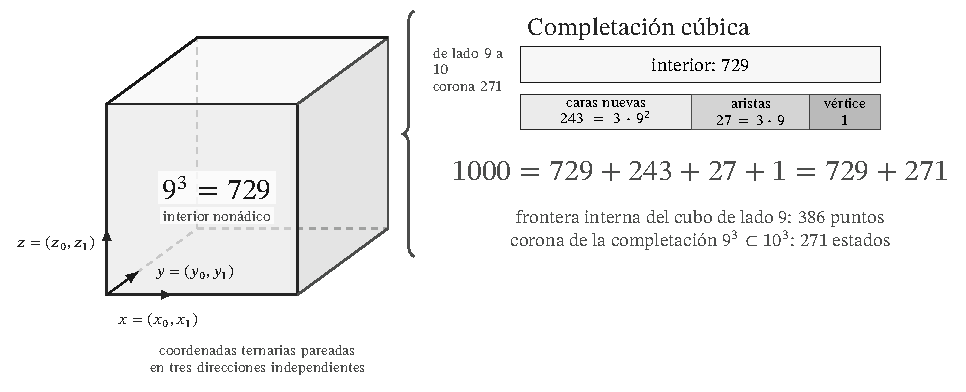
\includegraphics[width=\linewidth]{figures/cubo_emrh.pdf}
\caption{Representación cúbica de la ampliación de nueve a diez clases por coordenada. Los estratos \(S_1,S_2,S_3\) sitúan las incidencias añadidas en caras, aristas y ápice; sus cardinales forman la corona de \(271\) elementos. La frontera de \(386\) elementos pertenece al cubo inicial. La perspectiva geométrica complementa la partición de la figura~\ref{fig:revision-emrh}; las separaciones gráficas tienen función esquemática.}
\label{fig:completacion-cubo-recuperado}
\end{figure}


\subsubsection{Conservación de la unidad y compatibilidad dimensional}

La normalización no se limita a dividir una identidad aislada. En dimensión
\(d\), el producto \(\widehat E^d\) lleva la medida uniforme
\(\mu_d(\{x\})=10^{-d}\). La proyección coordenada
\(p_d:\widehat E^{d+1}\to\widehat E^d\) suprime la última coordenada.

\begin{proposition}[Compatibilidad proyectiva de las medidas normalizadas]
Para todo \(d\geq1\),
\[
 (p_d)_*\mu_{d+1}=\mu_d,
 \qquad \mu_d(\widehat E^d)=1.
\]
La masa del estrato con \(r\) coordenadas adicionales es
\(\binom dr9^{d-r}/10^d\), y la suma de las masas de todos los estratos
es uno.
\end{proposition}
\begin{proof}
Cada punto de \(\widehat E^d\) tiene diez preimágenes. Su masa total es
\(10\,10^{-(d+1)}=10^{-d}\). La igualdad para cualquier subconjunto
se obtiene sumando sobre sus puntos. La fórmula estratificada procede
del mismo recuento que \eqref{eq:revision-estratos}; el binomio
\((9+1)^d\) da la normalización total.
\end{proof}

En dimensión tres, retirar el ápice deja masa \(999/1000\), y
restituirlo añade \(1/1000\). Renormalizar antes de la restitución
definiría otra medida: la distinción es operacionalmente relevante.
En particular, conservación de masa probabilística, conservación de los
registros de transporte y disipación termodinámica son afirmaciones con
objetos diferentes. La proposición demuestra la primera y proporciona el
soporte compatible para estudiar la segunda; la tercera requiere una
realización dinámica y energética especificada.

También permanece diferenciada la frontera geométrica interna.
Sobre el representante cartesiano \(\{1,\ldots,9\}^3\), retirar
\(\{2,\ldots,8\}^3\) deja \(386\) puntos. Esta frontera pertenece al
cubo inicial, mientras \(\widehat C\setminus C\) pertenece a su
ampliación. La completación cúbica, la expansión posicional de base mil y
la lectura de incidencia excepcional comparten datos del soporte;
sus mapas respectivos determinan qué información de esos datos utiliza
cada representación.


\subsection{Incidencia cúbica y realización lorentziana}

La completación cúbica aporta una relación entre interior y frontera.
Su geometría puede desarrollarse mediante la incidencia de las seis caras
con los ocho vértices. Etiquetemos las caras por \((i,\varepsilon)\),
\(i\in\{1,2,3\}\), \(\varepsilon\in\{+1,-1\}\), y los vértices por
\(\nu\in\{+1,-1\}^3\). La matriz de incidencia es
\[
 M_{(i,\varepsilon),\nu}=\mathbf1_{\{\nu_i=\varepsilon\}}.
\]
Sean \(u=(1,\ldots,1)^{\mathsf T}\in\RR^6\), \(R_F\) la oposición de
caras y \(P_u=uu^{\mathsf T}/6\), \(P_-=(I-R_F)/2\).

\begin{proposition}[Cociente de incidencia de dimensión cuatro]
El Gramiano de incidencia satisface
\[
 MM^{\mathsf T}=12P_u+4P_-.
\]
Sus autovalores \(12,4,0\) tienen multiplicidades \(1,3,2\).
En consecuencia,
\[
 Q_\square=\RR^6/\ker(MM^{\mathsf T})
 \simeq\RR u\oplus E_-,\qquad E_-=\operatorname{im}P_-.
\]
\end{proposition}
\begin{proof}
Una cara contiene cuatro vértices; dos caras opuestas tienen intersección
vacía, y dos caras distintas no opuestas comparten dos vértices.
La matriz \(12P_u+4P_-\) tiene precisamente esas entradas.
El espacio uniforme tiene dimensión uno; las diferencias entre caras
opuestas generan un espacio de dimensión tres, ortogonal al uniforme.
Su complemento tiene dimensión dos y pertenece al núcleo.
\end{proof}

La descomposición \(1+3\) procede de la incidencia. La elección temporal
se declara mediante la forma bilineal
\[
 B_\square([x],[y])=\langle x,(P_--P_u)y\rangle.
\]
Está bien definida en el cociente, porque ambos proyectores anulan el
núcleo. En la base
\[
 t=[u]/\sqrt6,\qquad
 d_i=[e_{i,+}-e_{i,-}]/\sqrt2,
\]
su matriz es \(\operatorname{diag}(-1,1,1,1)\). Quedan explicitados
el dominio, la descomposición y la convención de signo que producen
la realización de Minkowski. El Gramiano positivo determina el cociente;
la asignación temporal determina la forma indefinida sobre él.

El operador
\[
 W_\square=\sqrt6P_u+\sqrt2P_-,\qquad
 W_\square e_{i,\varepsilon}=t+\varepsilon d_i
\]
envía las seis etiquetas de cara a direcciones nulas, puesto que
\(B_\square(t+\varepsilon d_i,t+\varepsilon d_i)=-1+1=0\).
La inversión de una dirección y la oposición de caras disponen así
de una realización geométrica concreta.

\subsubsection{Soldadura, inversión y subdivisión}

La realización celular utiliza un transporte invertible \(U_m(a)\),
que conserva la forma lorentziana, entre las fibras de los extremos de
una arista dual orientada \(a\), una etiqueta
de cara \(\lambda_m(a)\) y una orientación \(\sigma_m(a)\).
Con \(\ell_m=\ell_0/9^m\), la aplicación de soldadura es
\[
 \beta_m(a)=\ell_m\sigma_m(a)
 W_{\square,s(a)}e_{\lambda_m(a)}.
\]
La inversión compatible satisface
\[
 \beta_m(\bar a)=-U_m(a)\beta_m(a).
\]
Identifiquemos las fibras del origen en dos niveles consecutivos mediante
la isometría de refinamiento declarada. Si los nueve subsegmentos
\(a_1,\ldots,a_9\), de nivel \(m+1\), conservan la etiqueta
y la orientación al ser transportados a esa fibra común, entonces
\begin{equation}
 \beta_m(a)=\sum_{j=1}^9
 U_{m+1}(a_1\cdots a_{j-1})^{-1}\beta_{m+1}(a_j).
 \label{eq:soldadura-refinamiento}
\end{equation}
Cada término transportado equivale a \(\ell_m/9\) por la misma
dirección nula, lo que demuestra la identidad. La hipótesis de
compatibilidad determina qué subdivisiones realizan este refinamiento.
La ecuación reúne dirección, escala y transporte, en lugar de limitar
la correspondencia geométrica a un recuento de dimensiones.

Fijadas además la orientación y la forma lorentziana, la dualidad de
Hodge en \(\Lambda^2Q_\square^*\) satisface \(\star^2=-I\).
En dimensión cuatro, el signo es \((-1)^{2(4-2)+1}=-1\).
Se obtiene una estructura compleja real sobre las dos-formas y,
tras complejificación, los subespacios propios de valores \(+i\) y
\(-i\). La realización electromagnética utilizará este dominio
después de construir la sección electrónica y declarar su acoplamiento.

\subsection{Compatibilidad entre las reducciones modular y posicional}

La base decimal por bloques interviene mediante una división euclídea
que conserva simultáneamente residuo y cociente:
\[
 n=1000q+r,\qquad 0\le r<1000.
\]
Puesto que \(1000\equiv1\pmod9\) y \(1000\equiv1\pmod3\),
\[
 n\equiv q+r\pmod9,\qquad n\equiv q+r\pmod3.
\]
Por tanto, la reducción de un bloque requiere la contribución del
cociente para recuperar la clase del entero. Los números \(0\) y
\(1000\) tienen el mismo resto por \(1000\), pero clases diferentes
por \(9\) y por \(3\). Ésta es una razón operatoria para conservar
la memoria durante el cambio de resolución.

El refinamiento ternario y la determinación de un prefijo decimal
pueden coordinarse mediante un único residuo entero. Si \(N/3^L\)
es un extremo de cilindro y \(D/1000^r\) un extremo decimal, definimos
\[
 A=1000^rN-D3^L.
\]
Al añadir seis símbolos ternarios, \(N'=729N+\nu\),
\(L'=L+6\), con \(0\le\nu<729\). Si el prefijo decimal permanece
fijo, se obtiene
\[
 A'=729A+\nu1000^r.
\]
Si se incorpora además un bloque decimal \(\delta\), entonces
\(D'=1000D+\delta\), \(r'=r+1\), y
\begin{equation}
 A'=729000A+\nu1000^{r+1}-729\delta3^L.
 \label{eq:residuo-dos-bases}
\end{equation}
Ambas identidades se demuestran sustituyendo las definiciones. La
comparación de extremos se reduce así a operaciones enteras que
retienen la contribución de cada prolongación. Esta compatibilidad
es la que permite refinar una región antes de evaluar su coordenada real.

% Incorporación al final de extension.tex; no contiene una sección principal.
% Procedencia: RESULTADO_RECUPERADO; explicitación sectorial de las hipótesis.
% Fuentes leídas: monografía Doble proyección holográfica (cantera editorial),
% manuscrito/local/01_tesis_recuperada.tex y
% manuscrito/generated/algebra_holonomica.tex, especialmente §§1--7 y 21.
% Definición rectora de número: manuscrito/flattened/main_autosuficiente.tex,
% secciones que comienzan en líneas 22137 y 23000 de la cantera de 775 páginas.
% No se adopta su presentación global como prueba de todas las flechas TPK.

\subsection{El número como sección compatible y el valor como lectura}
\label{hist:seccion}

La distinción entre estado y observación permite precisar qué objeto se
prolonga cuando aumenta la resolución. A profundidad \(n\), sea \(X_n\)
el conjunto de estados admisibles producidos por APP--TRIT--TPK. Sus datos
incluyen posición, hojas suma y producto, residuos y cocientes, régimen,
orientación, acarreo, fase, ruta, frontera, memoria y supervivencia. No son
coordenadas independientes: las evaluaciones aritméticas y los transportes
anteriores imponen sus relaciones. Una prolongación conserva esas relaciones
en cada antecedente, aunque añada nuevos pasos y nuevos datos de memoria.
Éste es el sentido de la aritmética de historias que se desarrolla de forma
autosuficiente en este artículo.

Sean \(r_{m,n}:X_m\to X_n\), para \(m\geq n\), las restricciones de
profundidad, con \(r_{n,n}=\operatorname{id}\) y
\(r_{\ell,n}=r_{m,n}\circ r_{\ell,m}\). Cada restricción conserva el
prefijo y la información ya determinada en él.

\begin{definition}[Sección numérica compatible]
Un número HMT es una historia compatible del sistema de estados:
\begin{equation}
 x=(x_n)_{n\geq0}\in X_\infty:=\varprojlim_n X_n,
 \qquad r_{m,n}(x_m)=x_n.
 \label{hist:limite-inverso}
\end{equation}
Un lector es una operación adicional sobre un dominio especificado de estas
historias. Una cifra es una observación finita; un valor escalar es una
evaluación del lector. El par formado por la sección y su lector constituye
una presentación leída, no una redefinición de la identidad de la sección.
\end{definition}

En el dominio arquimediano \(X_\infty^{\mathrm{Arch}}\), el lector asocia
a cada prefijo un cilindro cerrado, conserva su encajamiento y hace tender
su diámetro a cero. Así determina
\begin{equation}
 \operatorname{ev}_{\mathbb R}:X_\infty^{\mathrm{Arch}}\longrightarrow
 \mathbb R,\qquad
 \{\operatorname{ev}_{\mathbb R}(x)\}=\bigcap_n I_n(x).
 \label{hist:evaluacion}
\end{equation}
La construcción concreta de estos cilindros y la decisión de sus fronteras
se desarrollan en la sección~\ref{sec:generacion}. La definición
\eqref{hist:limite-inverso} no afirma por sí sola que la imagen de
\eqref{hist:evaluacion} sea toda la recta: una afirmación de cobertura
requiere su propio teorema. Tampoco una igualdad de valores establece, sin
un resultado de inyectividad, la igualdad de sus historias. Esta separación
permite hablar de precisión como profundidad conservando la diferencia
entre el antecedente aritmético y su realización escalar.

\subsection{Composición de historias y multiplicador de memoria}
\label{hist:algebra}

Fijemos un sector de estados a profundidad \(n\) y una categoría
\(\mathcal C\) cuyas flechas sean sus historias admisibles. La composición
se escribe \(vu=v\circ u\): primero se recorre \(u\) y después \(v\).
Los pasos elementales proceden de la selección, el transporte y la
actualización del TPK. Una fibra trítica local admite la escritura
\(\mathbb R[J_x]/(J_x^2+\tau(x)1_x)\), donde
\(\tau(x)\in\{+1,0,-1\}\). El régimen y la orientación pertenecen al
estado que se transporta; una transición entre regímenes no equivale a
identificar sus álgebras cuadráticas.

La siguiente formulación precisa un sector algebraico de esa composición.
Para cada objeto \(x\), se da un álgebra real asociativa unitaria \(A_x\),
que puede ser no conmutativa. Para cada \(u:x\to y\), se da un
homomorfismo unital \(\rho_u:A_x\to A_y\). Suponemos una acción estricta:
\begin{equation}
 \rho_{\operatorname{id}_x}=\operatorname{id}_{A_x},\qquad
 \rho_v\rho_u=\rho_{vu}.
 \label{hist:accion-estricta}
\end{equation}
Para cada pareja componible \(u:x\to y\), \(v:y\to z\), fijamos un
multiplicador central invertible
\(\Omega(v,u)\in Z(A_z)^\times\). Se exige la normalización
\(\Omega(\operatorname{id}_y,u)=\Omega(u,\operatorname{id}_x)=1_y\)
y, para cada triple componible, la identidad
\begin{equation}
 \rho_w\bigl(\Omega(v,u)\bigr)\Omega(w,vu)
   =\Omega(w,v)\Omega(wv,u).
 \label{hist:cociclo}
\end{equation}
Son hipótesis explícitas sobre los transportes y sus coeficientes, no una
consecuencia de llamar holonómica a la dinámica. Al aplicar esta presentación
a un sector TPK deben identificarse sus \(\rho_u\) y \(\Omega(v,u)\).
Las transiciones expresadas mediante bimódulos requieren conservar esa
estructura y no quedan reemplazadas por \eqref{hist:accion-estricta}.

El espacio de sumas finitas
\[
 \mathcal H(\mathcal C,A,\rho,\Omega)
   =\bigoplus_{u\in\operatorname{Mor}(\mathcal C)} A_{t(u)}T_u
\]
recibe el producto bilineal
\begin{equation}
 (aT_v)(bT_u)=a\rho_v(b)\Omega(v,u)T_{vu},
 \label{hist:producto}
\end{equation}
si las flechas son componibles, y cero en otro caso. Aquí \(t(u)\)
designa el estado terminal. La suma reúne historias con coeficientes; el
producto concatena historias conservando el multiplicador del registro.

\begin{proposition}[Asociatividad sectorial con multiplicador central]
Bajo \eqref{hist:accion-estricta} y \eqref{hist:cociclo}, el producto
\eqref{hist:producto} es asociativo. Si el conjunto de objetos es finito,
su unidad es \(\sum_x1_xT_{\operatorname{id}_x}\).
\end{proposition}
\begin{proof}
Para \(u:x\to y\), \(v:y\to z\), \(w:z\to t\), sean
\(a\in A_y\), \(b\in A_z\), \(c\in A_t\). Los dos coeficientes
de \(T_{wvu}\) son
\begin{align*}
 ((cT_w)(bT_v))(aT_u):\quad&
 c\rho_w(b)\Omega(w,v)\rho_{wv}(a)\Omega(wv,u),\\
 (cT_w)((bT_v)(aT_u)):\quad&
 c\rho_w(b)\rho_w\rho_v(a)\rho_w(\Omega(v,u))\Omega(w,vu).
\end{align*}
La acción estricta iguala \(\rho_w\rho_v(a)\) con \(\rho_{wv}(a)\).
La centralidad de \(\Omega(w,v)\) permite desplazarlo a la derecha de
ese factor; \eqref{hist:cociclo} iguala entonces los productos restantes.
No se permutan los coeficientes \(a,b,c\). Si el triple no es componible,
ambas parentizaciones son cero por sus estados iniciales y terminales.
La bilinealidad concluye la prueba. Las identidades locales y la
normalización de \(\Omega\) verifican la unidad indicada.
\end{proof}

El acarreo del calendario proporciona un ejemplo efectivo. En la categoría
de un objeto y flechas \(C_9\), tomemos coeficientes
\(A=\mathbb R[z,z^{-1}]\), acción identidad y
\[
 \Omega(b,a)=z^{c_0(a,b)},\qquad
 c_0(a,b)=\left\lfloor\frac{a+b}{9}\right\rfloor,
 \quad 0\leq a,b<9.
\]
Las dos sumas de acarreos de un triple son
\(\lfloor(a+b+c)/9\rfloor\); por ello se cumple
\eqref{hist:cociclo}. La variable formal \(z\) registra la vuelta sin
asignarle un valor numérico. Imponer después \(z^{12}=1\) recupera el
registro dodecafásico del calendario \eqref{eq:extension108}; conservar
\(z\) sin esa relación distingue vueltas sucesivas. El ejemplo realiza
la memoria de este calendario, sin identificarla con la totalidad de la
memoria TPK.

\subsection{Doble varianza del refinamiento y conservación de la unidad}
\label{hist:doble-varianza}

Al restringir estados se prolongan observables en sentido contrario.
Consideremos las álgebras de funciones, con producto puntual,
\(D_n=\operatorname{Fun}(X_n,\mathbb R)\). La precomposición define
\begin{equation}
 r_{m,n}^*:D_n\longrightarrow D_m,
 \qquad r_{m,n}^*f=f\circ r_{m,n}.
 \label{hist:precomposicion}
\end{equation}
Son morfismos unitales; son además inyectivos cuando las restricciones
correspondientes son sobreyectivas. El límite directo
\(D_{\mathrm{cyl}}=\varinjlim_n(D_n,r_{n+1,n}^*)\) reúne las
observaciones de profundidad finita. No se identifica aquí este álgebra
con toda el álgebra de rutas: prolongar los operadores de transporte exige
también sus compatibilidades con el refinamiento.

\begin{lemma}[Unidad y naturalidad de la evaluación]
Si \(e_x\) es el indicador de \(x\in X_n\), se cumple
\begin{equation}
 r_{m,n}^*e_x=\sum_{y:\,r_{m,n}(y)=x}e_y,
 \qquad r_{m,n}^*1_n=1_m,
 \label{hist:unidad}
\end{equation}
y, para todo \(f\in D_n\), \(y\in X_m\),
\[
 \langle r_{m,n}^*f,y\rangle=\langle f,r_{m,n}y\rangle.
\]
Cada sección \(x\in X_\infty\) determina una evaluación bien definida
\(D_{\mathrm{cyl}}\to\mathbb R\), dada por \([f]\mapsto f(x_n)\)
para \(f\in D_n\).
\end{lemma}
\begin{proof}
Las fibras de \(r_{m,n}\) forman una partición de \(X_m\). Sus
indicadores son ortogonales y suman \(1_m\), lo que prueba
\eqref{hist:unidad}. La naturalidad es la definición de precomposición.
Finalmente, \((r_{m,n}^*f)(x_m)=f(x_n)\), de modo que dos representantes
compatibles dan la misma evaluación en el límite directo.
\end{proof}

La unidad global es la función constante uno sobre todas las posibilidades;
la sección individual selecciona una historia compatible. Conservar la
primera no significa inmovilizar la segunda. El refinamiento puede aumentar
la cantidad de extensiones y la profundidad de cada historia manteniendo
la unidad y todas las evaluaciones de sus antecedentes.

\subsection{Retorno de fase, representación de Weyl y dos lecturas}
\label{hist:puente-lecturas}

La ley \eqref{eq:holonomia-memoria} adquiere una realización operatoria
en la suspensión bilateral que se construirá en la
sección~\ref{sec:generacion}. Allí \(T\) es el avance de un paso,
\(V_9\) observa la fase nonádica, \(W_\delta\) la fase de rotación y
\(D_M\) el grado de memoria. Escribiendo
\(\widehat\Gamma_9=T^9\) para la vuelta en esta representación,
las relaciones de Weyl \eqref{eq:weyl-relojes} implican, sobre vectores
de soporte finito,
\begin{equation}
 \begin{aligned}
 V_9\widehat\Gamma_9&=\widehat\Gamma_9V_9,\qquad
 W_\delta\widehat\Gamma_9=e^{2\pi i9\delta}
     \widehat\Gamma_9W_\delta,\\
 [D_M,\widehat\Gamma_9]&=\widehat\Gamma_9.
 \end{aligned}
 \label{hist:tres-retornos}
\end{equation}
La primera igualdad sigue de \(\zeta_9^9=1\); la segunda, de nueve
aplicaciones de la covariancia de \(W_\delta\); la tercera expresa
el incremento unitario de memoria. La fase finita retorna, mientras la
rotación irracional y la memoria distinguen el estado siguiente. Los
caracteres y el parámetro \(\delta\) se realizan después desde la
construcción numérica allí especificada: no seleccionan retrospectivamente
las semillas. Esta representación describe observables y traslaciones de
la suspensión; no reemplaza todas las coordenadas ni todos los operadores
del TPK.

La doble lectura prolonga la misma distinción entre historia y observable.
En su dominio arquimediano se aplica \eqref{hist:evaluacion}; en el
dominio incidencial enriquecido, los mapas \(Q_n\) de la
sección~\ref{exc:doble-lectura} conservan las palabras y los marcos de
frontera. La igualdad allí demostrada
\(r_{n,m}Q_n=Q_mp_{n,m}\) determina su prolongación \(Q_\infty\).
Sobre el dominio común de ambas lecturas pueden considerarse conjuntamente
\(\operatorname{ev}_{\mathbb R}(x)\) y \(Q_\infty(x)\): la
primera retiene el valor; la segunda, la incidencia transportada que su
codominio conserva. La sección antecede a ambas. Esta articulación permite
pasar de la aritmética de historias a las constantes y a la lectura
excepcional sin convertir sus realizaciones en nuevos datos iniciales.

